\section{Training and Evaluation Protocol}
\label{sec:train}

\subsection{Training modes}

Two training modes are supported and can be toggled in the config:

\begin{description}
  \item[\texttt{windowed\_debug}] Fixed-length 288-step windows (24~h), batch size 32.
    Used for rapid iteration and smoke tests.  Does not maintain streaming state across windows.
  \item[\texttt{stateful\_stream}] Per-participant streaming with truncated BPTT over
    6-hour chunks, batch size 8.  The patient state is initialized once from $h_0$ and the
    timeline is walked in chunks; the carried state is detached at chunk boundaries.
    This is the default training mode for the AI-READI full-cohort run.
\end{description}

Training uses the Mamba-2 SSD Triton backend on CUDA; the sequential and chunked pure-PyTorch
backends produce identical forecasts and serve as CPU fallbacks for smoke tests and evaluation
on CPU-only machines.

\subsection{Objective}

The total loss keeps forecasting primary:
\begin{equation}
  \mathcal{L} = \mathcal{L}_{\text{pinball}}
  + \lambda_{\text{slope}}\mathcal{L}_{\text{slope}}
  + \lambda_{\text{shape}}\mathcal{L}_{\text{shape}}, \label{eq:loss}
\end{equation}
where $\mathcal{L}_{\text{pinball}}$ is the multi-horizon quantile loss over scored anchors.
The dose-ordering causal ranking term $\alpha\sum_a \mathcal{L}^a_{\text{rank}}$ from the
T1DEXI model is \textbf{disabled} for AI-READI
(\texttt{insulin\_ranking\_loss: disabled\_for\_aireadi}) because timed insulin
dose/IOB columns are not available as model inputs.

\subsection{Training convergence}

Figure~\ref{fig:training_curves} shows train and validation pinball loss over the 10-epoch
\texttt{stateful\_stream} run.  Loss converges steadily with no sign of over-fitting;
the best validation epoch was \bestValEpoch{} (best val pinball \bestValPinball~mg/dL).

\begin{figure}[h]
\centering
\IfFileExists{figures/generated/training_curves.png}{%
  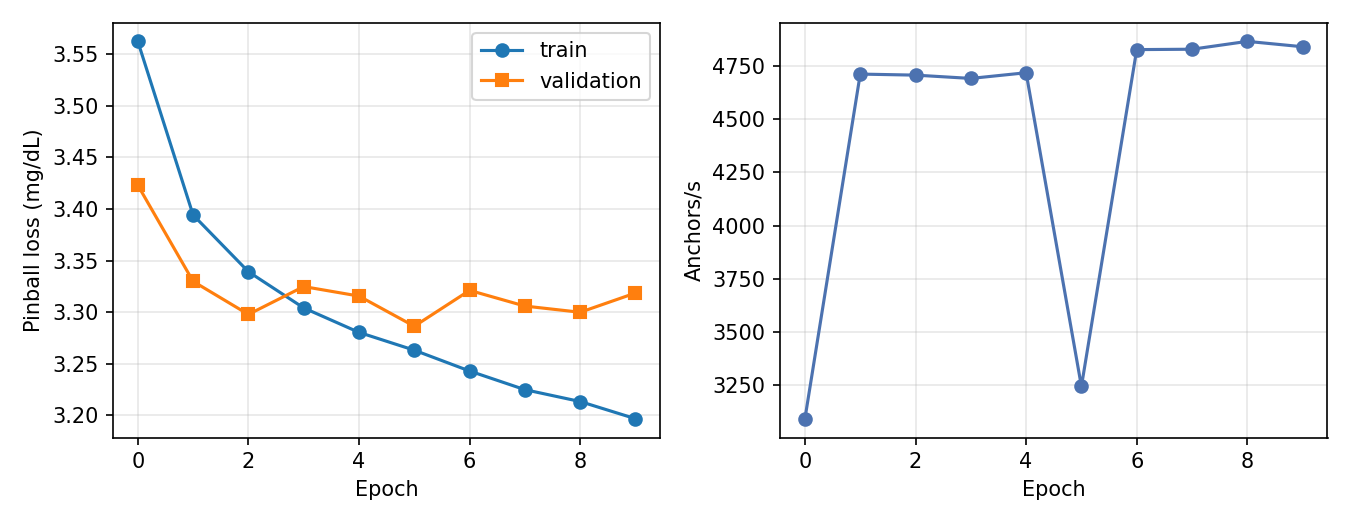
\includegraphics[width=0.9\textwidth]{figures/generated/training_curves.png}%
}{%
  \fbox{\parbox{0.85\textwidth}{\centering\vspace{1.2cm}
    \textit{[Figure: training and validation loss curves --- run make\_report\_figures.py]}
    \vspace{1.2cm}}}%
}
\caption{(A)~Train and validation pinball loss (mg/dL) over 10 epochs for the
  \texttt{stateful\_stream} run.  (B)~Training throughput (anchors/second) per epoch.
  Loss converges stably; per-epoch throughput is consistent under the chunked BPTT schedule.}
\label{fig:training_curves}
\end{figure}

\subsection{Evaluation modes}
\label{sec:evalmodes}

Five evaluation modes are reported with explicit labels to prevent confusion:

\begin{description}
  \item[\textbf{forecast-only} (deployable)] No future covariates are revealed to the decoder.
    This is the \emph{deployable} lower bound.
  \item[\textbf{factual-future} (retrospective upper bound)] The patient's actual future
    wearable values are revealed, as they would be in retrospective analysis.
  \item[\textbf{meal\_proxy}] The \texttt{predmeal\_flag} proxy is revealed as a planned
    scenario.  Directionally uncertain; not a validated causal intervention.
  \item[\textbf{activity\_proxy}] HR/steps/stress proxies are revealed.  Interpretable as
    a planned exercise session proxy; no hard causal sign.
  \item[\textbf{sleep\_rest\_proxy}] Sleep-stage flags are revealed.  Useful for
    overnight segment forecasting.
\end{description}

\noindent\textbf{Personalization} is evaluated at warm-up lengths
$w \in \{0, 6, 12, 24, 48\}$~h using an evidence-weighted per-user offset adapter.

\noindent\textbf{Subgroup evaluation} stratifies by
\texttt{participants\_study\_group}, \texttt{hba1c\_percent\_baseline},
\texttt{bmi\_baseline}, \texttt{participants\_clinical\_site}, \texttt{med\_insulin},
and \texttt{med\_any\_diabetes\_drug}.
